\documentclass[11pt]{./config/iiir}
\usepackage[numbers,compress]{natbib}
\usepackage[utf8]{inputenc}
\usepackage[english]{babel}
\usepackage{hyperref}
\usepackage{datetime}
\usepackage{xcolor}
\usepackage{amsmath}

\hypersetup{
  linkcolor  = black!70!black,
  citecolor  = blue!70!black,
  urlcolor   = blue!70!black,
  colorlinks = true,
}

\hyphenpenalty=100000 % To avoid hyphenation altogether
\sloppy % Force margin break 

\addto\captionsenglish{% Replace "english" with the language you use
  \renewcommand{\contentsname}%
    {Contents}%
}

\let\proglang=\textsf
\let\code=\texttt
\newcommand{\pkg}[1]{{\fontseries{b}\selectfont #1}}

\newdateformat{monthyeardate}{%
  \monthname[\THEMONTH] \THEYEAR}
  
\providecommand{\tightlist}{%
  \setlength{\itemsep}{0pt}\setlength{\parskip}{0pt}}

  \iiir[yssp]{yy}{nnn}{\monthyeardate\today}

\iiauthor{Hadi (\href{mailto:hadi@iiasa.ac.at}{\nolinkurl{hadi@iiasa.ac.at}}) \protect\footnotemark[1]{}, Second Author \protect\footnotemark[2]{}, Third Author \protect\footnotemark[1]{}}

\protect\footnotetext[1]{International Institute for Applied Systems Analysis (IIASA).}\protect\footnotetext[2]{Second author affiliation.}

\iititle{Line One of Title:\\Line Two After Linebreak or Use Only Line1 and Allow Title to Break
Automatically}

\iiapproved{ Program Leader Name (\href{mailto:name@iiasa.ac.at}{\nolinkurl{name@iiasa.ac.at}})}{Leader}{IIASA Program}

\begin{document}

\iicoverpage

\iifrontsection{Foreword}Edit or remove this text.

\iifrontsection{Acknowledgments}Edit or remove this text.

  \iifrontsection{About the Authors}
    \subsection*{Hadi}Some text about the first author. Edit or remove this text.
    \subsection*{Second Author}Some text about the second author. Edit or remove this text.
    
  
\iifrontsection{Abstract}This template demonstrates some of the basic you'll need to create your
IIASA Working Paper or YSSP report combining \proglang{R} markdown and
\proglang{LaTex}.

\iitableofcontents{Contents}



\iilistoffigures

\iibody

\section{Introduction}\label{introduction}

Markdown documents are fully reproducible and work with several
programming languages (e.g.~Python, SQL), for more details see
\citep{RStudio:2016, GitHub:2014}.

\section{Code formatting}\label{code-formatting}

\subsection{Using Latex commands}\label{using-latex-commands}

Use the latex commands:

\begin{itemize}
\tightlist
\item
  Programming language \proglang{R}
\item
  Package or library \pkg{plyr}
\item
  Code snippets \code{print("abc")}
\end{itemize}

\subsection{Using code chuncks}\label{using-code-chuncks}

Code can be inserted in the text using grave accent ( \(\grave{}\) ),
e.g. \texttt{x=1}, or in markdown blocks, such that

\begin{verbatim}
> x <- seq(1, 10, length.out = 100)
> round(x,2)
\end{verbatim}

\begin{verbatim}
  [1]  1.00  1.09  1.18  1.27  1.36  1.45  1.55  1.64  1.73  1.82  1.91
 [12]  2.00  2.09  2.18  2.27  2.36  2.45  2.55  2.64  2.73  2.82  2.91
 [23]  3.00  3.09  3.18  3.27  3.36  3.45  3.55  3.64  3.73  3.82  3.91
 [34]  4.00  4.09  4.18  4.27  4.36  4.45  4.55  4.64  4.73  4.82  4.91
 [45]  5.00  5.09  5.18  5.27  5.36  5.45  5.55  5.64  5.73  5.82  5.91
 [56]  6.00  6.09  6.18  6.27  6.36  6.45  6.55  6.64  6.73  6.82  6.91
 [67]  7.00  7.09  7.18  7.27  7.36  7.45  7.55  7.64  7.73  7.82  7.91
 [78]  8.00  8.09  8.18  8.27  8.36  8.45  8.55  8.64  8.73  8.82  8.91
 [89]  9.00  9.09  9.18  9.27  9.36  9.45  9.55  9.64  9.73  9.82  9.91
[100] 10.00
\end{verbatim}

The chunk can also include plot commands, which crete and insert the
figures in the the text, such as Figure \ref{fig:simple-r-plot} produced
by the following chunk

\begin{verbatim}
> y <- cos(x)
> plot(x, y, type = "l", col = "red")
> lines(x, -y, col = "blue")
\end{verbatim}

\begin{figure}[ht]

{\centering 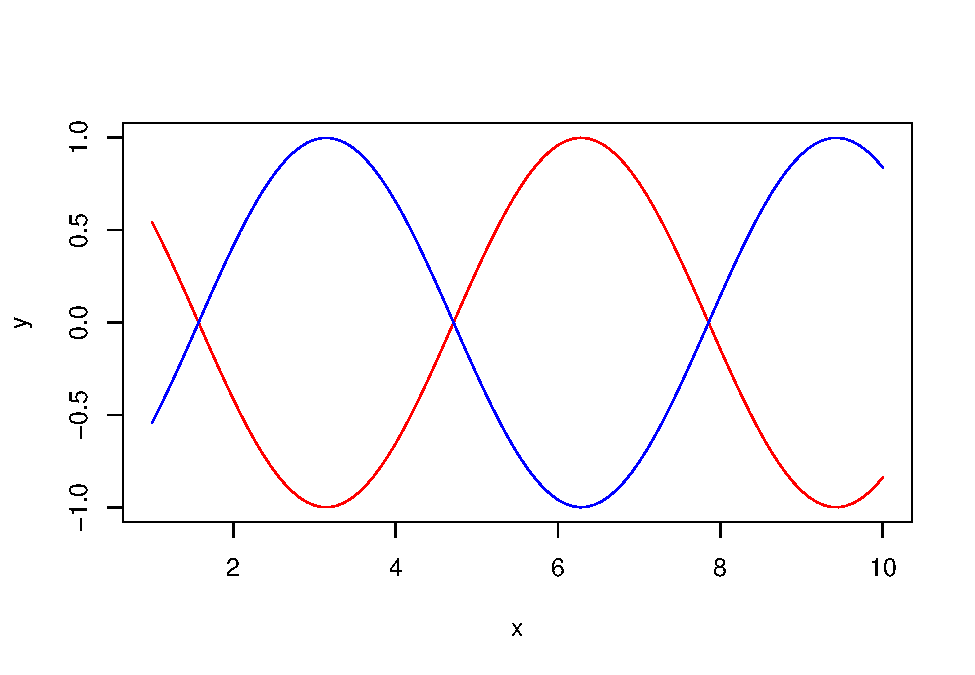
\includegraphics{yssp_report_Hadi_files/figure-latex/simple-r-plot-1} 

}

\caption{\proglang{R} plot example. For \code{LaTex} code in the caption use double backslash \textbackslash\textbackslash.}\label{fig:simple-r-plot}
\end{figure}

For more details see the package
\href{./inst/doc/iiasaRmarkdown.pdf}{vignette} and the following web
tutorials \url{http://rmarkdown.rstudio.com/index.html} and
\url{https://guides.github.com/features/mastering-markdown/}.

\bibliographystyle{unsrtnat}

\bibliography{references}


\end{document}


